\chapter{Phân tích nhiều chiều dữ liệu thang đo định lượng}


Nội dung này được tham khảo và tổng hợp từ các tài liệu tham khảo  .....

\section{Kiem dinh Pearson}
\subsection{Ham phan phoi tich luy}
\begin{equation}
    F(x) = P(X<x)
\end{equation}
% Mỗi hình một caption
\begin{figure}[h]
    \centering
    % Hình thứ nhất
    \begin{minipage}{0.45\textwidth}
        \centering
        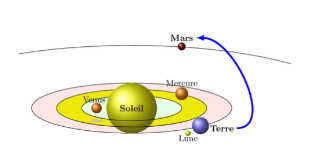
\includegraphics[width=\textwidth]{../../assets/images/figure-2.png}
        \caption{Hình 1}
        \label{fig:image1}
    \end{minipage}
    \hfill
    % Hình thứ hai
    \begin{minipage}{0.45\textwidth}
        \centering
        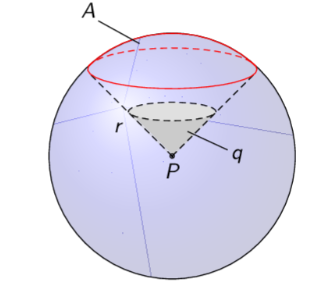
\includegraphics[width=0.7\textwidth]{../../assets/images/figure-3.png}
        \caption{Hình 2}
        \label{fig:image2}
    \end{minipage}
\end{figure}

% Hai hình 1 caption

\begin{figure}[h]
    \centering
    % Hình thứ nhất
    \begin{minipage}{0.45\textwidth}
        \centering
        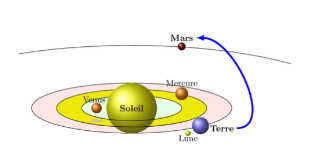
\includegraphics[width=\textwidth]{../../assets/images/figure-2.png}
          \end{minipage}
    \hfill
    % Hình thứ hai
    \begin{minipage}{0.45\textwidth}
        \centering
        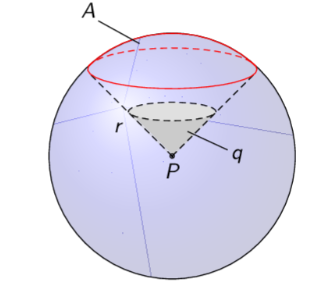
\includegraphics[width=0.7\textwidth]{../../assets/images/figure-3.png}
    \end{minipage}
    \caption{Hình đôi}
        \label{fig:image3}
\end{figure}
\subsection{Tiểu mục 2}

%%%%%%%%%%%%%%%%%%%%%%%%%%%%%%%%%%%%%%%%%%%%%%%%%%
% nội dung này có thể tham khảo giáo trình ĐSTT và HH2
\section{Mục 2}
\subsection{Tiểu mục 1}

\subsection{Tiểu mục 2}

\noindent % Để loại bỏ thụt lề đầu dòng
\begin{minipage}{0.4\textwidth} % Phần hình ảnh (40% chiều rộng trang)
    \centering
    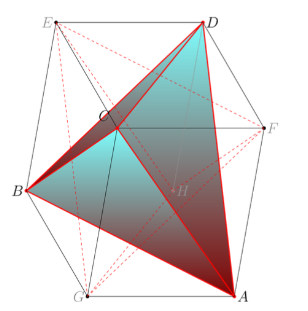
\includegraphics[width=\textwidth]{../../assets/images/figure-1.png} % Đường dẫn tới ảnh
    \captionof{figure}{Hình minh họa} % Chú thích cho hình
    \label{fig:image}
\end{minipage}%
\hfill % Thêm khoảng cách giữa hình và chữ
\begin{minipage}{0.55\textwidth} % Phần văn bản (55% chiều rộng trang)
    Đây là đoạn văn bản mô tả hình ảnh. Bạn có thể viết bất kỳ nội dung nào ở đây để giải thích hoặc chú thích cho hình bên cạnh. Sử dụng phần trăm chiều rộng hợp lý để tối ưu bố cục tài liệu.
\end{minipage}
%%%%%%%%%%%%%%%%%%%%%%%%%%%%%%%%%%